\chapter{Implementation} \label{cpt-implementation}

Our case study is based on an implementation within the framework \emph{Diligent Engine}.[@TODO: cite DiligentEngine]
This framework includes a multi-\ac{API} rendering backend, with modern integrations for \ac{GPU}-driven rendering.
One of these modern features is the support for mesh shading in Microsoft's D3D12 rendering \ac{API}. 
The support for modern rendering features while still maintaining access to all core features, makes 
\emph{Diligent Engine} a good place to start from. For the case study, we enhanced the mesh shading pipelin 
to better fit our purposes of drawing a huge amount of voxels. We also made small changes to the integrated 
view-frustum culling, which was updated to work on meshlet-groups rather than meshlets themselves. This change 
was made during the restructuring of the draw tasks. The updated pipeline changes how meshes are dispatched 
because of the use of additional acceleration structures. This chapter provides an overview of all the changes and 
additions to the framework and how the pipeline works in specific. The implementation details can be found in the 
appendix \ref{cpt-appendix}.

\section{Pipeline Initialization} \label{sec-piepline-initialization}

\begin{figure}[h]
    \centering
    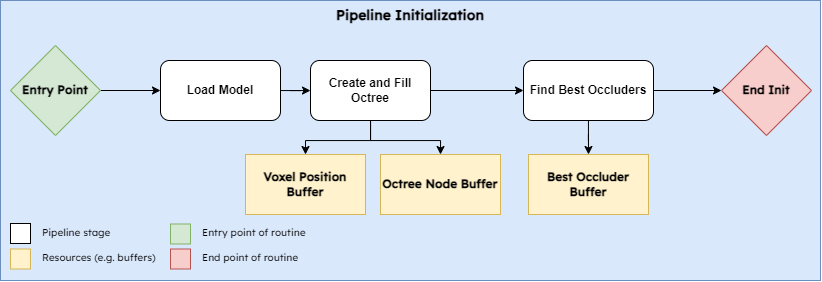
\includegraphics[width=\linewidth]{images/graphics/pipeline-initialization.png}
    \caption{The initialization process of the rendering pipeline. Depending on the voxel model, an octree node 
    can hold anything between zero and \emph{n} voxels, \emph{n} being the amount of threads per threadgroup}
    \label{fig:pipeline-initialization}
\end{figure}

\noindent
The pipeline is, as usual, split into an initialization routine and an update loop. The initialization is 
called once during the beginning of the execution flow and the render loop is initiated after the initialization 
finished. Then, the loop is continuously called - once per frame. Figure \ref{fig:pipeline-initialization} shows 
the initialization procedure. 

\subsection*{Voxel Model Loading} \label{subsec-voxel-model-loading}

For the purpose of this case study, a single, solid voxel mesh is loaded, but this could as well be a scene 
consisting of multiple solid voxel models. In our implementation, the positions of voxels inside a regular 
grid are loaded, skipping grid cells, where no voxels are located. For loading the voxels, the tool \emph{binvox} 
is used \cite{binvox, Nooruddin2003}. 


\subsection*{Octree Creation} \label{subsec-octree-creation}

After loading any voxel model, an octree is created that covers 
the complete scene - in this case the bouding volume of the voxel model. As discussed in chapter 
\ref{subsec-highres-svo-dags}, it is recommended to use a highly efficient and compressed octree 
implementation like an \ac{SVO} or a Sparse Voxel \ac{DAG} \cite{Kampe2013}. For the purpose of our case 
study, we used a custom octree implementation which refers to indices in a global \emph{voxel position buffer}, 
as shown in figure \ref{fig:voxelpos-octreenode-buffer}.\\

\begin{figure}[h]
    \centering
    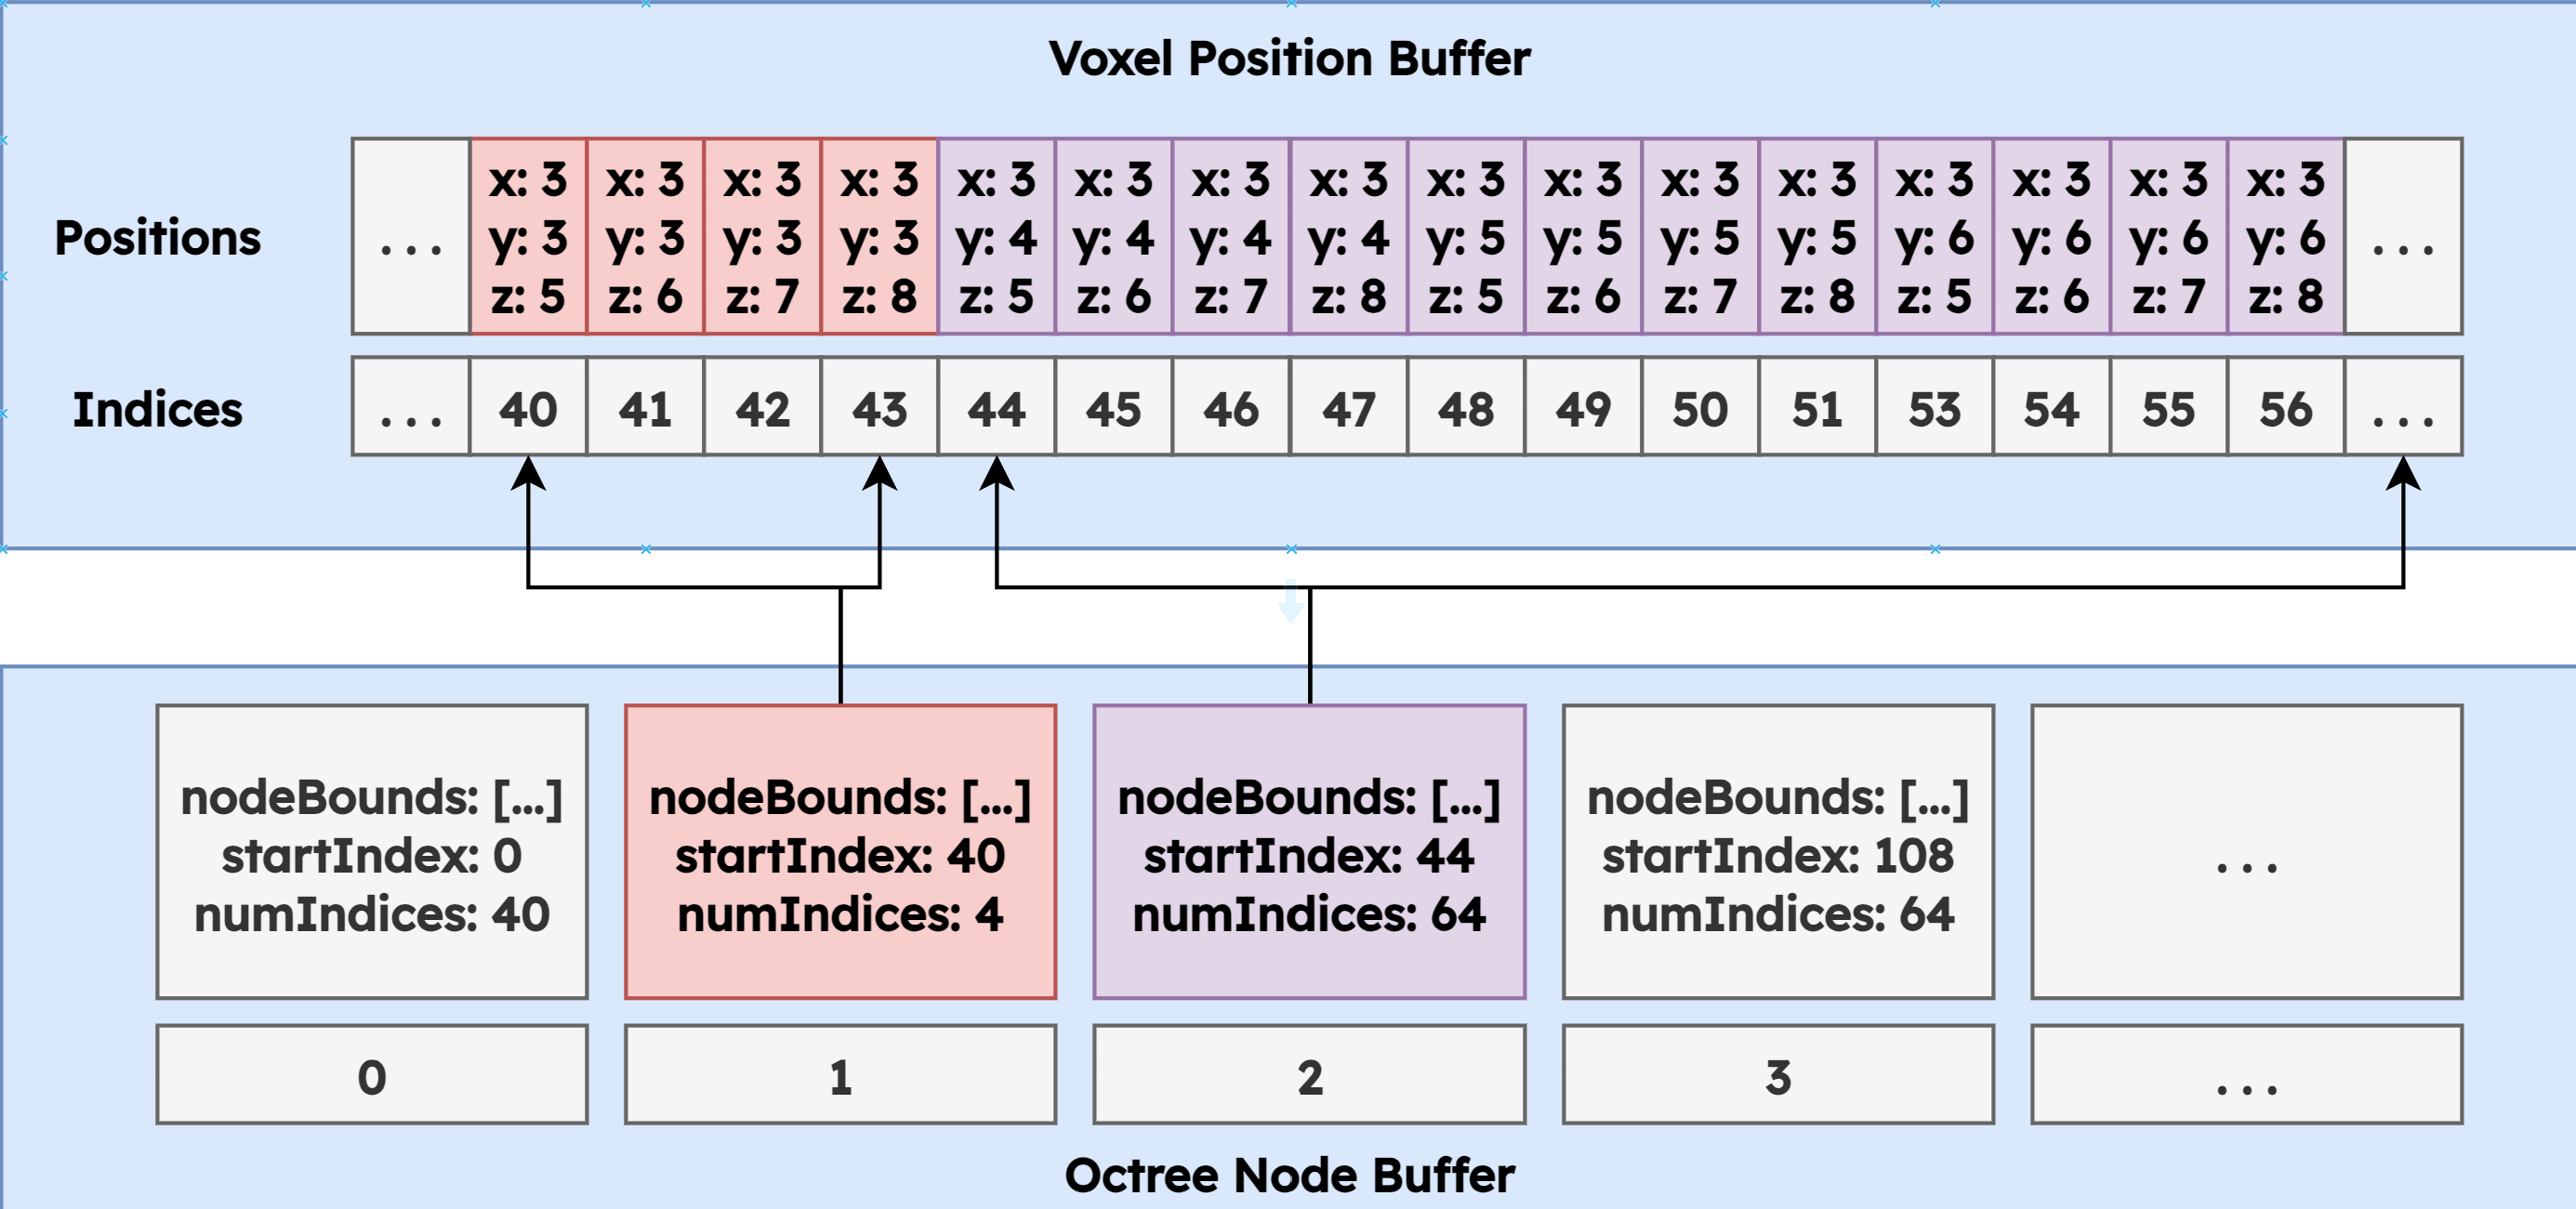
\includegraphics[width=\linewidth]{images/graphics/voxelpos-octreenode-buffer.png}
    \caption{The voxel position buffer and the octree node buffer. The latter one providing a 
    specific structure to the first one.}
    \label{fig:voxelpos-octreenode-buffer}
\end{figure}

\noindent
Since the \ac{GPU} is supposed to generate a lot of voxels on the fly, data buffers like the voxel position buffer 
need to be considered.
For structuring the data, various options are available. A first approach involves the voxels being layed 
out as individual meshlets, which was our initial idea. This means that individual voxels can be culled and 
each \ac{GPU} thread generates one voxel. This would mean that only the voxel position buffer is needed. 
The amplification shader takes the positions, culls meshlets against the view-frustum and dispatches the 
mesh shader with the given data. As long as no spatial container like an octree is used, this approach works 
fine. When considering the use of an octree, however, another layout serves better. In this case, each \ac{GPU} 
threadgroup takes care of one octree node, with the maximum amount of voxels per node being equal to the 
amount of threads per threadgroup. Using this layout, each thread in a threadgroup again takes care of one 
voxel. The octree node information now can store additional information, which can be used for octree node 
based view frustum culling. To generate this data, the octree is queried during the initialization, resulting 
in an extra \emph{octree node buffer} which stores an index into the voxel position buffer and a count of voxels,
associated with the node. After sorting the voxel position buffer, this additional structure identifies voxel 
positions that are located adjacent to each other inside an octree node. Figure \ref{fig:voxelpos-octreenode-buffer} 
shows the data layout and how it relates to the voxel position buffer. 


\subsection*{Best Occluder Selection} \label{subsec-best-occluder-selection}

The next step in the initialization procedure is to pre-compute the best occluders. This part is a significant one, 
since it computes important data for the occlusion culling. As mentioned in chapter \ref{subsec-two-pass-occlusion-culling},
best occluders are usually specifically authored by artists during the creation of the scene. This process is only 
possible, if the models are static in a sense, that they do not change in size or shape. An alteration like this 
could result in inefficient occlusion queries or even the elimination of occluders altogether. In the context of 
volumetric scene representations, where voxel models are often a target of manipulation by players or physical 
interactions, a predetermination of best occluders is not possible in the way it is for static models.
This specific scenario is what our approach aimes for, and why the next step in the pipeline pre-processes best 
occluders. Note, that this implementation does not include an update of the best occluders. It only serves as a 
case study of the occlusion culling algorithm. Updating the best occluders when the voxel model is altered, 
needs to be evaluated seperatly, but is considered to be trivial for occasional changes to the mesh. A more 
demanding change to the octree content is given when computing physical interactions within the duration of a frame.
In this case, further test need to be done to evaluate the impact on performance. \\

\noindent
To find the best occluders, different constraints need to be considered. Our approach makes use of the inner, non-visible 
voxels, and approximates them using the octree. This means, an octree node is equivilent to a best occluder, if:

\begin{itemize}
    \item the maximum number of voxels per octree node is a power of three (e.g. $2^{3}$,  $3^{3}$, ...),
    \item the number of voxels present within the node is equal to the maximum number of voxels per octree node,
    \item and the octree node's boundary is equal to the \emph{minimal convex hull} of all voxels within the node.
\end{itemize}

\noindent
In practice, this means, that best occluders are given, if the octree node is completely, tightly filled 
with voxels. If the octree node, however, is larger than the block defined by the maximum number of voxels 
per node, this block cannot be approximated correctly by the bounds of the node. This property of a best 
occluder is propagated up the tree, as long as all eight child nodes satisfy the requirements of being a 
best occluder. During the depth pre-pass, the best occluders are drawn as "large voxels" which are the size 
of the respective best occluder node. This can be achieved by simply reusing the mesh shader used in the 
normal draw call, and inputting the node's position and bounds. This way, a whole node gets drawn, instead 
of the individual voxels, reducing the computation cost for the best occluders by at least \emph{n} times, 
with \emph{n} being the maximum amount of voxels per node. The best occluders are seperatly stored in a 
buffer, so they can be dispatched efficiently. \\

%[@TODO: Add data structure diagram of best occluder buffer]
%[@TODO: add images]

\noindent
This concludes the initialization of the pipeline. When changes are applied to the voxel data, the voxel buffer,
the octree node buffer and the best occluder buffer need to be updated accordingly. Alternatively, the best 
occluders can be implicitly calculated on the basis of the octree node buffer. This would make the best 
occluders buffer redundant but would result in a higher dispatch count with a lot of discarded nodes, 
where the criteria for best occluder are not met. Since all computations are more or less in parallel, this 
will not affect frametimes for a moderate amount of octree nodes. Nevertheless, since we are using static 
voxel models with no runtime alternation, a static, pre-calculated buffer for best occluders is used.


\section{Rendering Loop} \label{sec-rendering-loop}

\begin{figure}[h]
    \centering
    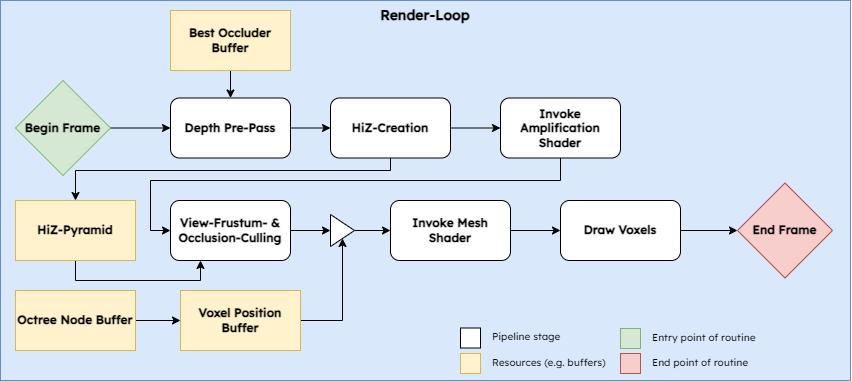
\includegraphics[width=\linewidth]{images/graphics/render-loop.png}
    \caption{The rendering loop of the rendering pipeline.}
    \label{fig:pipeline-loop}
\end{figure}

\noindent
The rendering loop consists of three main steps: The depth pre-pass including \ac{HiZ} generation, the 
amplification shader and the mesh shader. The different stages consume and generate various data buffers 
and textures, as shown in figure \ref{fig:pipeline-loop}. 

\subsection*{Depth Pre-Pass} \label{subsec-depth-prepass}

The frame computation starts by computing the depth pre-pass, which is the custom render pass central 
for the occlusion culling. In this pass a compute shader is invoked that takes the best occluders and 
draws them to the depth buffer. This depth pass does not draw to the back buffer, making the computation 
relatively efficient. It can also include optional computations like frustum culling for further 
optimization. This can be effective when there are a lot of nodes in the best occluders buffer. 
Consequently, the depth buffer has data from possible occluders and the \ac{HiZ} generation is started. 
The z-pyramid is generated by another compute shader, which samples four texels of the input texture 
(the full resolution depth buffer) and outupts the lowest z-value to an outupt texture (mip level 1). 
This chain of mip-maps is shown as the [@TODO: here is a jump from mip lvl 1 to full z-pyramid!]
\ac{HiZ}-pyramid in figure \ref{fig:pipeline-loop}.


\subsection*{The Amplification Shader} \label{subsec-amplification-shader}

Now, the amplification shader is invoked, each threadgroup resembling one octree node. The amplification 
shader now decides over which meshlets are drawn. Here, view frustum culling is applied to a threadgroup 
and the occlusion culling is executed by projecting the boudning box of the meshlets onto the view plane 
and querying the \ac{HiZ}-pyramid for depth values. If the voxel position is found to be visible - or not 
occluded by the best occluders - the position is added to the payload, ready to be drawn by the mesh shader. 


\subsection*{The Mesh Shader} \label{subsec-mesh-shader}

The mesh shader executes the appropriate transformations, constructs a uniform voxel around the voxel position 
and outputs the geometry. The voxels in a \ac{GPU}-Driven approach can be completely generated on the \ac{GPU}, 
minimizing the memory bandwidth used per frame. This optimization technique is not only efficient, but also 
trivial for uniform, static voxel geometry. When dispatching one voxel per thread, one voxel corresponds 
to one meshlet, making pre-computation completely redundant, as opposed to the common precomputation of meshlets, 
as mentioned in chapter \ref{sec-mesh-shading}. 


\section{Something along the lines of "specific example"} \label{sec-todo}

[@TODO: Check if I should explain mip levels in chptr 4]

- Where can I put the initial thought of having voxels as meshlets? -> maybe motivation? 
- Early-z rejection vs. our approach



// --------------------------------------------------------------------------------- //
Motivation:
Use Meshlet Culling in voxel rendering to optimize GPU Driven Voxel Rendering


Implementation Considerations:

- Meshlet Culling at first, then problem, because meshlet culling algorithm depends on different algos
    - Meshlet Backface Culling -> Not possible because Meshlets are voxels in this case
    - Meshlet Occlusion Culling -> Using 2 Pass Depth Occlusion Culling sounds good!
    - 2PDOC relies on drawing best occluders which are usually hand picked by artists (buildings)
        -> We can dynamically pick best occluders by selecting full octree nodes as best occluders!

- Optimize octree by using High Res SVOs (https://www.cse.chalmers.se/~uffe/HighResolutionSparseVoxelDAGs.pdf).
    - As shown in the paper, here we also only need to encode if a node is filled or not. This way we can 
    optimize memory and proccessing speed! (Not done here because of limitation in loading and voxelizing models.)

- Explain why Mesh Shading is useful here and what the differences to HiZ and Two-Pass OC are!


- Limitations: 
- Worse performance on slopes? -> Check and measure!
- Align octree bounds with outer most voxel bounds, so no misalignment happens!

- (Larger nodes which are not being split can be "full" without being full!)

// --------------------------------------------------------------------------------- //
